

\chapter{Differentiating between BPMN, CMMN and DMN}
\label{chapter:indicators}

\todo{Ausblick, was bietet dieses Kapitel und was ist das Ziel}
\todo{Diagramme mit Legende versehen} 

\section{BPMN and routine processes}
\label{section:BPMNindicators}
Creating business process diagrams nowadays almost seems to be intuitive. This results from a broad background of routine process modeling incorporating the rise and fall of BPR, ARIS and its EPCs and many more routine process modeling languages. Altogether, they formed the current understanding of business process management and modeling. 
Since BPMN is a broadly adopted modeling language and a standard that shaped the industry, users might be mislead when to use BPMN correctly. In this chapter, a definition of requirements and indicators will be provided for the correct use case scenario identification in terms of BPMN as well as a short introduction to the model. 

\begin{sidewaysfigure}

	\centering
	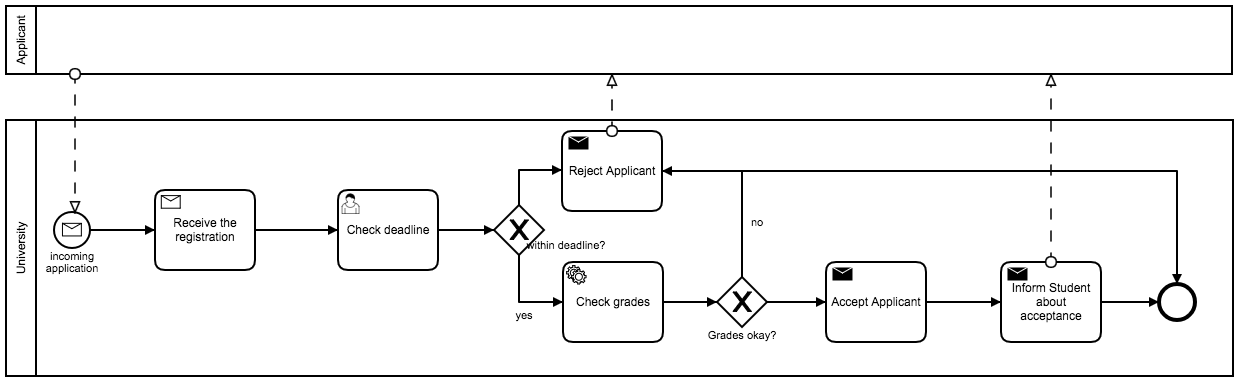
\includegraphics[scale=0.5]{../figures/chapter_indicators/BPMN_Example_Student_Application.png} 
		\caption{A small BPMN example: the application process for study programs.}
	\label{fig:BPMNex}
\end{sidewaysfigure}

Business Process Model and Notation incorporates \textit{Business Process}, which has been defined and redefined many times by today. For this thesis, we use the OMG's definition of business processes: 
\begin{quote}
Business Processes: business plans include Courses of Action - what the enterprise has to do to achieve its Ends - transformed into Business Processes that ecnompass activities, sequencing, dependencies, interactions, triggering by business events, etc. \cite{bmm2015}
\end{quote}

Business processes are ways to achieve goals, to align activities along them and to define interactions, decisions and events. This definition basically incorporates all the core elements of BPMN: Activities, paths, swimlanes (for responsibilities), decisions and events. To recap the notation of BPMN, a small example is shown in figure \ref{fig:BPMNex}. 
In this model, the application process for a student program is shown, which consists of tasks such as \textit{Receive the registration} or \textit{Check deadline}. Tasks can be precised as \textit{Manual tasks}, \textit{Send / Receive Tasks} and have assignees, as shown in \textit{Check deadline}. In current Workflowmanagementsystems, this workflow model can be fully automated and the assignee is presented its tasks when they are instantiated, e.g. when an application form was received. BPMN models have a starting and an end point which can also be events. In our example, the starting point is a \textit{Message Event}, that indicates the process has started due to a received message. 
Decisions are a major concern in every control flow oriented graph and BPMN models usually consist of several decision points. They are notated as diamond-shaped \textit{Gateways}, either empty or with a special symbol inside. Each symbol stands either for \textit{AND}, \textit{OR}, \textit{XOR} or \textit{COMPLEX}. Gateways direct the control flow depending on the decision logic prescribed. In our example, a \textit{XOR} Gateway controls the workflow into either the direction of acceptance or the opposite one, depending on what date the applicant's form was submitted. Additionally, the communication between the workflow's two participants is notated as so called \textit{Pools}, which can be divided into \textit{Swimlanes}. Each pool is a communication partner and a swimlane indicates different responsibilities such as departments. If a pool is not filled with BPMN elements, the communication partner is out of scope of the modeler and the processes cannot be modeled. These pools are \textit{Black boxes}. 

As we see in the example, the process is well-structured and has no room for creative decisions or even discussions at run-time. The only way the process can differ, is human intervention or changing the process at design-time. The former is equal to not executing the process in the intended way and the latter is bad for processes in volatile environments. BPMN is suited for a limited variety of processes, foremost business processes. The OMG's specification excludes specifically the following \cite{BPMNspec}: 

\begin{quote}

\begin{itemize}
\item Definition of organizational models and resources,
\item Modeling of functional breakdowns,
\item Data and information models,
\item Modeling of strategy,
\item Business rules models
\end{itemize}

\end{quote}

%Although excluded, data and information can be modeled by artifacts. It's not like an \textit{Unified Modeling Language} (UML) model where classes and inheritance is mapped, but it is useful to handle forms and different kind of documents which need to be passed along the tasks. 
%For business rules, this is also applicable. BPMN contains a special form of tasks called \textit{Business Rule Task}, which "[...] provides a mechanism for the Process to provide input to a Business Rules Engine and to get the output of calculations that the Business Rules Engine might provide" \cite{BPMNspec}. Business Rule Tasks are predestined for small spreadsheets fed injected into a business rule engine, which is usually a Java class. It is easy to use and implement, since the Business Analyst files a spreadsheet and the developer uses the CSV-file to implement the business rule engine. This procedure, however, works only at design-time and not at run-time, which is a downside being discussed in a subsequent section about DMN. 

Furthermore, the OMG's specification not only provides exclusions such as the ones mentioned above, but it helps to indicate the correct usage of BPMN. Derived from the background chapter \ref{chapter:background} and the example above, the following indicators (table \ref{tab:bpmnIndicatorsTable}) serve as a guidance for modelers to identify when to use BPMN correctly. 

% Please add the following required packages to your document preamble:
% \usepackage{booktabs}
% \usepackage{graphicx}
\begin{table}[]
\centering

\resizebox{\textwidth}{!}{%
\begin{tabular}{@{}ll@{}}
\toprule
Indicators                   & BPMN                                                                                                                                                                         \\ \midrule
General                      & \begin{tabular}[c]{@{}l@{}}Predefined sequences of activities with decisions (gateways) to direct the \\ sequence along the alternative paths or for iterations\end{tabular} \\
Type of process              & \begin{tabular}[c]{@{}l@{}}Predefined, fully specified, repeatable, business process, \\ control flow oriented\end{tabular}                                                  \\
Type of work                 & Routine work with possible automation                                                                                                                                        \\
Type of decisions            & Simple, driven by rules or events                                                                                                                                            \\
Control flow                 & Strict and necessary                                                                                                                                                         \\
Intervention at run-time     & no                                                                                                                                                                           \\
Typical application          & Value-added chain processes, workflows across companies, departments etc.                                                                                                    \\
Key question before modeling & \begin{tabular}[c]{@{}l@{}}Does the work consist of routine elements which can \\ be optimized or even automated?\end{tabular}                                               \\ \bottomrule
\end{tabular}%
}
\caption{BPMN indicators.}
\label{tab:bpmnIndicatorsTable}
\end{table}

Information about processes is often stored in documents, deprecated models or held by knowledge carriers according to Dumas et al. \cite{Dumas2013}. This information needs to be extracted by the application of the so called \textit{Process Discovery}, which is in short gathering all the information in a technical or manual way before creating the models. Having this information gathered together, the key question before modeling is \textit{Does the work consist of routine elements which can be optimized or even automated?} (see \ref{tab:bpmnIndicatorsTable}). Routine processes occur regularly and their flow is "known a priori" according to \cite{Zeising_2014}. Consequently it is not intended to change the process flow during run-time, as routine are well-structured and predefined. This is a major problem for workers whose job is more based on knowledge and their experience than routine work, wherefore is Case Management and CMMN were forged and standardized. 
In our example, the decisions are simple yes or no questions. One of them, \textit{Check grades}, is a business rule task containing a small table of when a grade acceptable or must be rejected. Overall, the decisions do not require modeling any requirements or personnel apart from the assignee involved in the decision making process. Furthermore, the decisions are always stuck with rules or events that happened before. The process itself is control-flow-oriented and the control flow is necessarily strict since every candidate needs to be processed in a fair and equal manner. In the end, the process could be automated completely with the appropriate workflowmanagementsystem and would not need any assignee to check the deadline or the grades. 
According to the indicators, the example is modeled using the suitable modeling language as the process was predefined and well-structured. To prove the indicators' validity, a use case example taken from the eKulturPortal GmbH \footnote{see \url{http://ekulturportal.de/}} is provided in chapter \todo{hier fehlt die Chapter referenzierung!}. 

\section{CMMN and knowledge work}
Routine work occurs in every company, every industry and even in our leisure time. However, not every job is comprised entirely of routine work. If a person is sick and needs to see the doctor, often the doctor's job consists of routine parts and ad hoc parts. Each patient suffers in a different way, has a private or statutory health insurance, is able to understand the doctor's language or not. In each case, the doctor or the medical personnel needs to decide in an ad hoc manner to identify the patient's disease and medicate him accordingly. Overall, this job requires more knowledge and experience than a strict workflow. Applying the BPMN indicators makes the necessity of a different modeling technique obvious as the indicators do not meet the requirements of this example (flexibility instead of a strict workflow, knowledge driven instead of control flow driven).
Standardized by the OMG in 2014 \cite{CMMNspec2014}, the modeling language is intended to meet the requirements of knowledge intensive professions and support workers with models and their execution in workflowmanagementsystems. 
The above described example diverges from the business processes explained in the BPMN section earlier. Instead of focusing on what \textit{has} to be done in which order, the medical personnel should adhere to what \textit{can} be done, as Van der Aalst et al. described in \cite{aalst2005}. This is an essential part of the \textit{Case Management} (CM) and \textit{Adaptive Case Management} (ACM) approach. Case management starts with a case such as a legal case, a patient's disease or "some other focal point around which actions are taken to achieve an objective" \cite{CMMNspec2014}. Each case contains a set of tasks and files necessary to achieve the goal. These sets are "minimally predefined" \cite{CMMNspec2014} resulting in two phases of working with cases: the design phase and the running phase \cite{CMMNspec2014}. During the design phase, tasks and information are aggregated in a manner that is very similar to business process designs. As a result, the work is available in a more structured way as it has been before yet with the possibility to perform the work in a completely ad hoc if necessary. Additionally, case management requires the run-time flexibility such as performing tasks depending on the situation, changing the order of tasks or even collaborate with different people involved as intended. 
At a first glance, this seems counter-intuitive since the common understanding of modeling processes is modeling business processes or similar strictly structured ones. To illustrate the paradigm of case management and introduce the CMMN notation, figure \ref{fig:CMMNex} provides an example \todo{soll hier noch eine Legende angelegt werden?}. The subsequent explanation is derived from \cite{CMMNspec2014} and \cite{hinkelmann2015}.

\begin{sidewaysfigure}

	\label{fig:CMMNex}
	\centering
	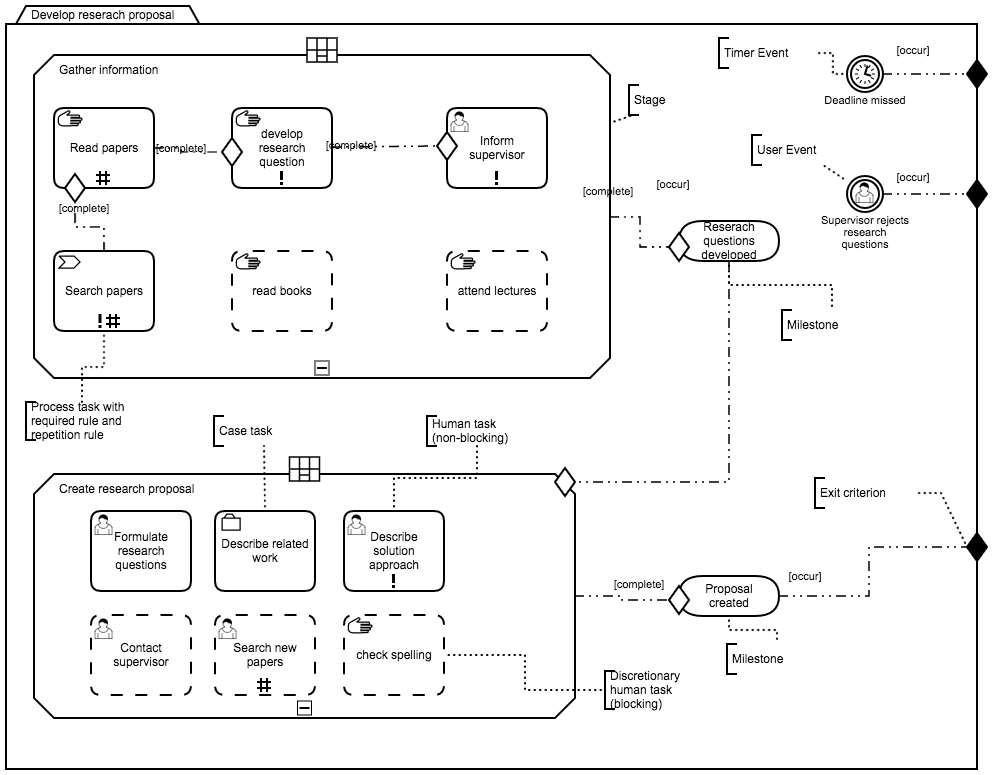
\includegraphics[scale=0.5]{../figures/chapter_indicators/CMMN_Example_Proposal_Creation.png} 
		\caption{CMMN example: Creating a research proposal.}
\end{sidewaysfigure}

The first element that immediately catches the eye in this example is a large folder depicting the \texttt{Case Plan Model}, a root element containing all further elements involved with a name tag in the upper right corner. Next, there is a big structure called a stage and illustrated as a rectangle. Similar to BPMN, stages form a group of elements into a sub process or - to put it in the CMMN context - in a sub case. Stages can be connected via sentries and connectors that are the lines between tasks and the diamond shaped exit or entry criteria. Both, exit and entry criteria trigger when events occur. There are three possibilities to make sentries trigger:
\begin{itemize}
\item \texttt{on [event] if [condition]} 
\item \texttt{on [ event]}
\item\texttt{if  [condition]}
\end{itemize}

According to the CMMN specification, this provides the opportunity to receive events and check whether they have effect on the following process steps \cite{CMMNspec2014}. In figure \ref{fig:CMMNex} a timing event is called \texttt{Deadline missed}. This event is connected to an exit criterion, denoted as a black diamond on the border of the Case Plan Model. When the event is triggered, the sentry checks \texttt{on [deadline missed] if [date today > deadline date]} \footnote{Note: This example is just for illustration purpose and incorporates no concrete syntax nor semantics.} and triggers the exit criterion terminating the case due to the missed deadline. A different event type is the \texttt{User Event} listening to user interactions that trigger the exit criterion. Besides these two event types, each task, stage and \texttt{Case File Item} can trigger events on their own which are received by sentries. \texttt{Case File Items} are containers for pieces of information, for instance the patient's record or in this example the papers which need to be read (not contained in the diagram). They are denoted as files known from the notation as computer files are depicted.
Another structural element is the \texttt{Milestone}, an oval shaped form representing an "achievable target" \cite{CMMNspec2014} and providing the ability to measure the progress of a case. Each milestone can have multiple entry criteria or none to show that a milestone is reached or not. In general, "no work is directly associated with a milestone" \cite{CMMNspec2014} but rather a "completion of a set of tasks" or "the availability of key deliverable" \cite{CMMNspec2014}. Figure \ref{fig:CMMNex} contains two example milestones: \texttt{Research questions developed} and \texttt{Proposal created}. Both milestones are connected to either a stage or an exit criterion indicating a dependency. The first milestone needs to be achieved to create the research proposal, the latter one determines the successful termination of the case. \\
As mentioned earlier, CM requires run-time flexibility and by now, there has nothing been explained but tasks, events and milestones which are per se inflexible. To guarantee run-time planning, tasks and stages have a discretionary version. Discretionary means, a user may decide during run-time if this task or stage will be executed in a following iteration. At this point, the knowledge and experience comes into play. In our example, the gathered papers might not be enough to provide good citations and emphasize the solution approach. Here,  only the writer himself can identify if he needs to do more research to find correct citations as this is a decision requiring knowledge and experience in writing research papers. It is to his or her discretion if the task will be executed or not. 
Supplementary to \texttt{Discretionary Items}, \texttt{Planning Tables} indicate the ability to plan \texttt{Discretionary Items} and apply control mechanisms called \texttt{Applicability Rules}. Case workers are presented \texttt{Planning Items} if the corresponding \texttt{Applicability Rule} evaluates to true. Overall, this allows the modeler and the case workers to plan at design-time (creating the case model) and at run-time (planning the time discretionary items). 
The last visible part of the CMMN notation that has not been explained is the type of tasks available. In the example case, there are four types of tasks (each type can be indicated in the upper right corner of the task):
\begin{itemize}
\item \texttt{Human Tasks} either blocking (indicated with a "User" in the upper right corner) or non-blocking with a hand in the right corner
\item \texttt{Process Task} with a "Chevron" symbol 
\item \texttt{Case Task} with a folder symbol 
\end{itemize}

Both \texttt{Human Tasks} indicate that an assignee with the appropriate role needs to fulfill the modeled work here. Non-blocking signifies this step can be done while other tasks of the model run simultaneously in contrast to the blocking one, which does not allow other tasks to be performed at the same time. A \texttt{Process Task} calls a simple business process modeled e.g. in BPMN and a \texttt{Case Task} calls a different case potentially independent from the one being executed. In figure \ref{fig:CMMNex}, \texttt{Read Papers} is a non-blocking human task, \texttt{read books} a non-blocking discretionary human task, \texttt{Formulate research questions} a blocking human task, \texttt{Describe related work} a case task and \texttt{Search papers} a business process task.
Apart from the mentioned types of tasks, there a additional execution semantics as seen in the \texttt{Search papers} task. An exclamation mark signifies this task as to perform, a sharp that this task has several iterations and a play symbol indicates the \texttt{Manual Activation Rule} (not in the example). This rule is connected to entry criteria and transitions from the status \texttt{enabled} to \texttt{active} if the criterion's condition is fulfilled. 
CMMN, in contrast to BPMN, offers a complete lifecycle with corresponding states. 

\begin{figure}
  \centering
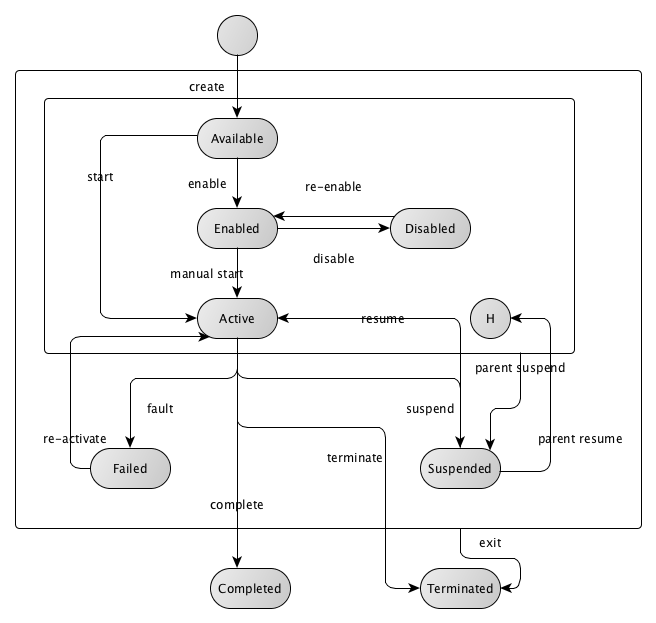
\includegraphics[width=0.7\textwidth]{../figures/chapter_indicators/CMMN_Stage_and_Task_Lifecycle_CMMN.png} 
\caption{Stage and Task Lifecycle according to figure 7.3 in the CMMN specification.}
  \label{fig:CMMNstates}
\end{figure}

Figure \ref{fig:CMMNstates} is a replica of figure 7.3 in \cite{CMMNspec2014} and shows the different states and transitions for stages and tasks. These stages, compared to BPMN, allow the modeler and the worker to measure and to plan work in a different way than business processes are handled. One of the most commonly mentioned downside of BPMN is the lack of states and transitions according to \cite{Recker2010}. In the example (fig. \ref{fig:CMMNex}), states are not included since they are not visible in the notation and only occur during run-time. In addition to fig. \ref{fig:CMMNstates}, CMMN offers similar states for sentries and the whole case plan model and can be found in the execution semantics chapter in \cite{CMMNspec2014}. \\

% Please add the following required packages to your document preamble:
% \usepackage{booktabs}
% \usepackage{graphicx}
% \usepackage[normalem]{ulem}
% \useunder{\uline}{\ul}{}
\begin{table}[]
\centering
\resizebox{\textwidth}{!}{%
\begin{tabular}{@{}ll@{}}
\toprule
Indicators                   & CMMN                                                                                                                                                                                                                                                            \\ \midrule
General                      & \begin{tabular}[c]{@{}l@{}}Workflow can be managed in a flexible way or in a complete \\ ad hoc manner, overall cast cannot be orchestrated by \\ predefined sequence of tasks\end{tabular}                                                                     \\
Type of process              & Depending on evolving circumstances, ad hoc, data centric                                                                                                                                                                                                       \\
Type of work                 & Ad hoc, not predefined, sparsely routine work                                                                                                                                                                                                                   \\
Type of decisions            & Stateful conditions, rules, exit and entry criteria                                                                                                                                                                                                            \\
Control flow                 & Not necessary but can be modeled                                                                                                                                                                                                                                \\
Intervention at run-time     & Yes                                                                                                                                                                                                                                                             \\
Typical application          & \begin{tabular}[c]{@{}l@{}}Patient care, medical diagnosis, insurance cases, \\ governmental permitting, problem resolution in call centers, \\ sales and operations planning, invoice discrepancy handling, \\ engineering of made-to-order products\end{tabular} \\
Key question before modeling & \begin{tabular}[c]{@{}l@{}}Does the work comprise unstructured elements and \\ ad hoc workflows requiring knowledge or \\ experience instead of strict rules?\end{tabular}                                                                                      \\ \bottomrule
\end{tabular}%
}
\caption{CMMN indicators.}
\label{tab:cmmnIndicatorsTable}
\end{table}

Table \ref{tab:cmmnIndicatorsTable} shows a summary derived from the explanation and the example, both planting on the basis of the CMMN specification \cite{CMMNspec2014}. The example emphasized that CMMN is in general applicable for not predefined, to a high degree knowledge dependent work. Decisions are modeled in conditions on when to enter or exit stages, task or milestones. Rules such as \texttt{Application Rule} or \texttt{Repetition Rule} allow the modeler to guide the case worker through tasks and show him or her what tasks have to be done and which have to be done for a specific amount of iterations. However, decisions similar to gateways in BPMN are not in scope of this notation and dedicated to the case worker. In addition, the required flexibility is fulfilled by \texttt{Discretionary Items} allowing the workers with the appropriate role to adapt the workflow in during run-time. States as shown in figure \ref{fig:CMMNstates} contribute to this flexibility but also let the involved personnel measure the progress of each case. This results in a more manageable and verifiable way of Case Management. 
\todo{italic zu Schreibmaschinen Style aendern}
\todo{korrigieren}

\section{DMN and decision making}
In section \ref{section:BPMNindicators} decision-making in BPMN was shown with the aid of a small example, whose excerpt is shown in figure \ref{fig:BPMNshortenedApplicationEx}. Two gateways guide the control flow according to the decisions made. Each gateway compares a value with a given limit and verifies it. If the value is correct, the control flow passes on to the next gateway or, in case the value is out of bounds, rejects the student's application. 
Figure \ref{fig:BPMNexpandedApplicationEx} demonstrates a more sophisticated version of the same process. Here, the the university has four requirements but only one needs to be fulfilled to pass the application process and to be accepted for the desired study program. All of the gateways are \texttt{OR} gateways signalizing it doesn't if one of these requirements is not met but one of the other is. At a first glance, figure \ref{fig:BPMNexpandedApplicationEx} looks more complicated than figure \ref{fig:BPMNshortenedApplicationEx}. Although the actual decision-making process is kept simple, the BPMN notation with its gateways makes it look confusing and, at a much larger scale, for the reader impossible to comprehend the process a whole. At this point, DMN becomes relevant. 

\begin{sidewaysfigure}
  \centering
    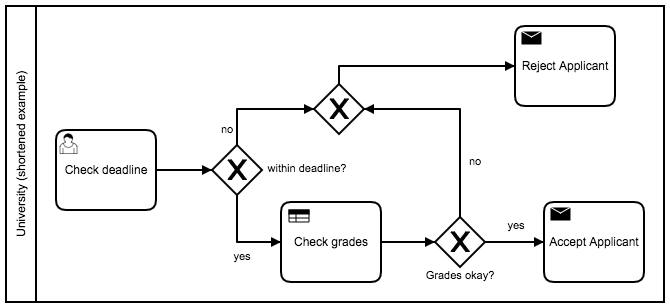
\includegraphics[scale=0.5]{../figures/chapter_indicators/BPMN_Example_Student_Application_Short.png}
    \caption{Shortened example from section \ref{section:BPMNindicators} with only two decisions.}
  \label{fig:BPMNshortenedApplicationEx}
    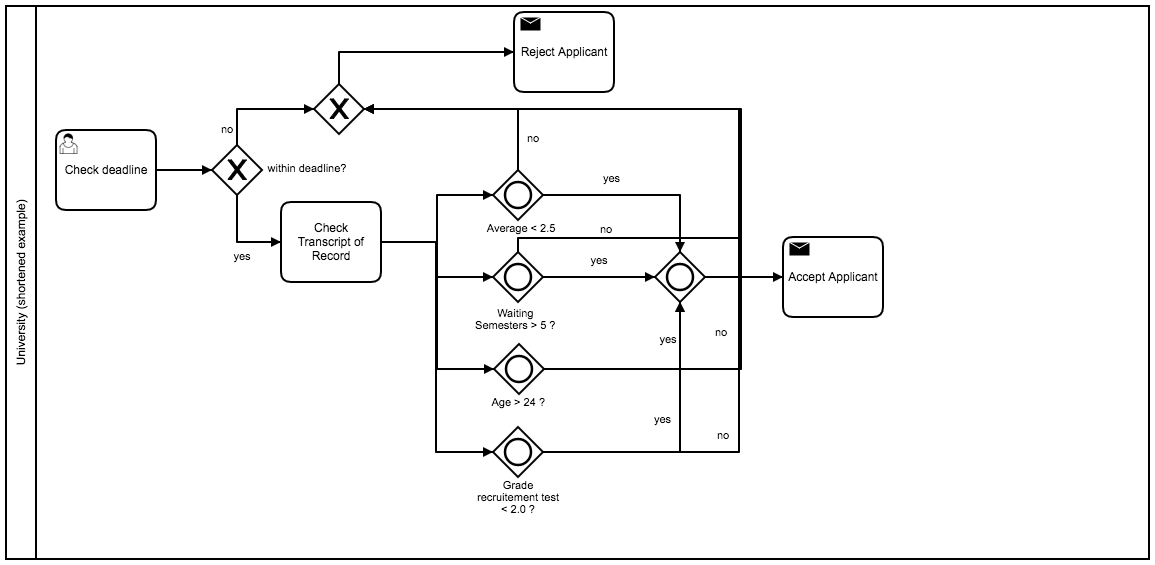
\includegraphics[scale=0.4]{../figures/chapter_indicators/BPMN_Example_Student_Application_DMN_Short.png}
    \caption{Shortened example from section \ref{section:BPMNindicators} with additional decisions.}
  \label{fig:BPMNexpandedApplicationEx}
\end{sidewaysfigure}

\begin{figure}
\begin{center}
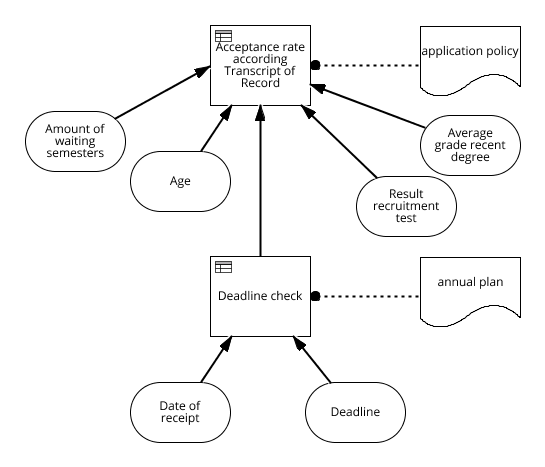
\includegraphics[width=0.5\textwidth]{../figures/chapter_indicators/DMN_Application_Example_Deadline_ToR.png} 
\end{center}
\caption{A DMN Decision Requirement Graph incorporating the decision-making of the BPMN process in \ref{fig:BPMNexpandedApplicationEx}.}
\label{fig:DMN_DRD_Application}
\end{figure}

The DMN notation comprises two parts: the \acl{DRG} with one ore more \aclp{DRD} and the decision tables. Figure \ref{fig:DMN_DRD_Application} illustrates the corresponding \ac{DRG} for the decision-making seen in fig. \ref{fig:BPMNexpandedApplicationEx}. DMN's notation for DRDs contains only four distinct shapes and three different types of connectors. In fig. \ref{fig:DMN_DRD_Application}, there are three elements provided and one is missing due to the shortness of the example: 
\begin{itemize}
\item \texttt{Decision}: Decisions are depicted as rectangles and incorporate the decision logic which is mapped in decision tables. In the example there are two decisions, \texttt{Deadline check} and \texttt{Acceptance rate according to Transcript of Record} and both have a table symbol in the upper right corner indicating the decision logic. 
\item \texttt{Input Data}: Each decision needs inputs and \texttt{input data} is the fundamental and least complex form possible. This element stores information of any type from simple types like dates and integers to lists and functions expressed via \acf{FEEL}. An \texttt{Input Data} element may only be connected directly to decisions and knowledge sources. 
\item \texttt{Knowledge Source}: DMN makes it explicit where knowledge sources are involved in the decision-making. Typically knowledge sources are documents, best practices but also people or bodies of legislation \cite{DMNspec2016}.  "Knowledge sources are the authorities for a decision [...]" \cite{DMNmicroguide}, which may be connected with input data since managers, for instance, might need background information not directly involved in the decision logic. In the example, the application policy and annual plan of the university is used as \texttt{knowledge source}.
\item \texttt{Business Knowledge Model}: In contrast to \texttt{Knowledge Sources}, \texttt{Business Knowledge Models} are non-authoritative and serve as container for analytic models, decision logic or business rules \cite{DMNspec2016}. It is depicted as a rectangle with cut-off corners in the upper left and lower right. As they only influence decisions directly, the specification allows consequently no connection but with decisions or different business knowledge models. 
\end{itemize}

As stated above, the notation comprises only four elements making it a very compact modeling language in terms of the \ac{DRG}. In addition, there are three different connectors indicating either an \texttt{information requirement} (connections from decisions to decisions or input data to decisions), an \texttt{authority requirement} (connections from knowledge models to decisions, business knowledge models or different knowledge sources) or \texttt{knowledge requirement} (connections from business knowledge models to decisions or different business knowledge models). 

\begin{sidewaysfigure}
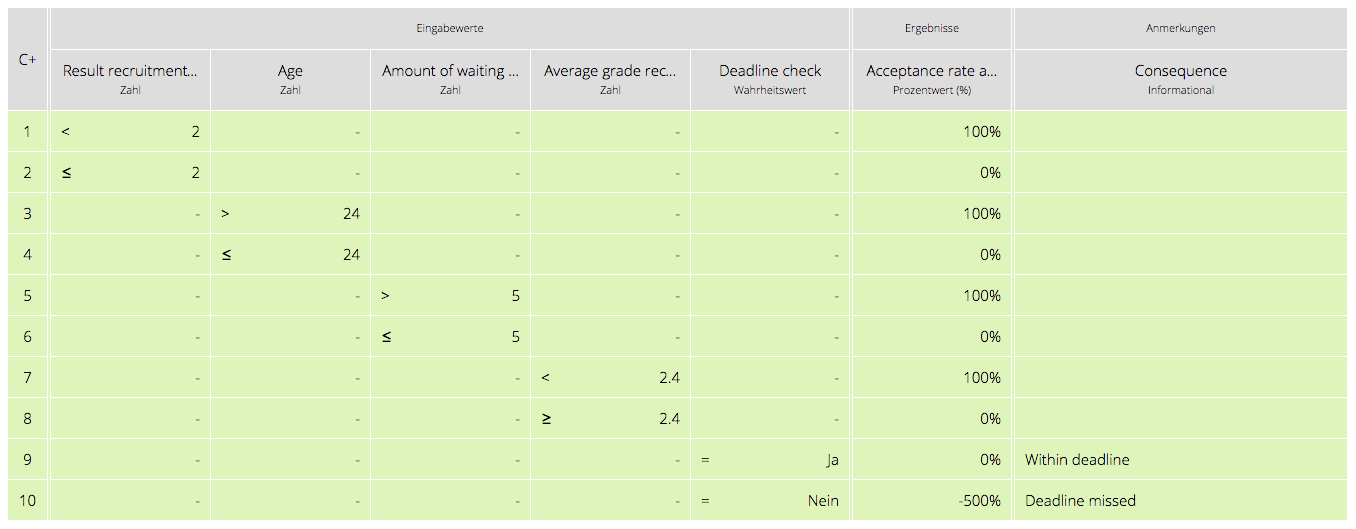
\includegraphics[width=\textwidth]{../figures/chapter_indicators/DMN_Application_Example_Decision_Table_ToR.png} 
\caption{An example DMN decision table with the decision logic accord to the BPMN example in fig. \ref{fig:BPMNexpandedApplicationEx}.}
\label{fig:DMN_decision_table_application}
\end{sidewaysfigure}

The second part of the DMN specification allows the modeler to create decision tables containing the decision logic. An example table \footnote{Each modeling tool implementing the DMN specification is allowed to vary the orientation of decision tables and the concrete look, such as colors or shades.} is provided in figure\ref{fig:DMN_DRD_Application} implementing the decision logic according to the BPMN example in figure \ref{fig:BPMNexpandedApplicationEx}. Each table comprises of several input columns and at least one output column. An input can be a string, integers, floats or basically any type of numbers required. In this example table, there are five inputs and one output with annotations such as \texttt{Deadline missed}. Each row signifies a rule in the following syntax: \texttt{If [INPUT A] AND [INPUT B] then [OUTPUT C]} \cite{DMNspec2016}. The inputs are logically connected by the boolean \texttt{AND}-operator resulting in as many outputs as desired, if a rule matches. For every input in the decision table, there is an \texttt{input data} element modeled in the related \ac{DRG}. This also applies for decisions and sub-decisions. 
Comparing the table with the BPMN example demonstrates a downside of the decision table: the "\texttt{AND} only" syntax. However, modeling \texttt{OR} connections is possible with a workaround. Besides the table's data and rules, business analysts can also define \texttt{hit policies}. These policies are necessary if some of the rules overlap. In the example table (fig. \ref{fig:DMN_DRD_Application}), all of the rules are intended to overlap making a hit policy necessary. There are two major categories of policies: \texttt{single hit} and \texttt{multiple hit}. The former one allows only to trigger one rule, the latter one allows several rules to trigger. A brief overview with an explanation can be found in table \ref{tab:DMN_hit_policies}. 

% Please add the following required packages to your document preamble:
% \usepackage{booktabs}
% \usepackage{graphicx}
\begin{table}[]
\centering
\resizebox{\textwidth}{!}{%
\begin{tabular}{@{}ll@{}}
\toprule
Policy       & Variations                                                                                                             \\ \midrule
Single hit   & Unique (no overlap allowed)                                                                                            \\
             & Any (overlap allowed, outputs must be equal)                                                                           \\
             & Priority (returns matching rule with highest output priority)                                                          \\
             & First (first hit by rule order)                                                                                        \\
Multiple hit & Output order (returns all hits in decreasing output priority order)                                                    \\
             & Rule order (returns all hits in rule order)                                                                            \\
             & \begin{tabular}[c]{@{}l@{}}Collect (aggregates all hits with specified operators:\\ sum, min, max, count)\end{tabular} \\ \bottomrule
\end{tabular}%
}
\caption{DMN hit policies cited from the DMN specification \cite{DMNspec2014}.}
\label{tab:DMN_hit_policies}
\end{table}
 
To achieve an \texttt{OR} connection of the rules, the hit policy \todo{DMN Tabelle probieren auf Englisch umzustellen} is set to \texttt{Multiple Hit: collect (sum)} and the measuring unit of the output is set to percentage. Consequently, the acceptance rate is measured in percentage. The applicant is able to achieve zero or more than 100 percent according to the \texttt{collect: sum} rule. Another problem of this method is the inflexibility of the outputs. In this example, an output value of \texttt{true} or \texttt{false} would have been the best way to model the decision, but neither the decision table nor \ac{FEEL} allow the aggregation of boolean values. 
Last of all to mention is the sub-decision \texttt{Deadline check}. The decision logic is not implemented in this table, but is referenced by a another decision table (see fig. \ref{fig:DMN_DRD_Application} for illustration). A simple check written in \ac{FEEL} counts the difference between the application's date of receipt and the given deadline. If the result is less then zero, the deadline is missed and the output of \texttt{Deadline check} \texttt{false}. Otherwise, if the result equals zero or more, the result it \texttt{true}. 
To individualize the decision logic or create more advanced rules, the DMN specification aggregated several functions and types into an expression language called \acl{FEEL}. It is similar to \ac{SQL} and \ac{PMML} making it easier to understand for non-developers. The expression used in the \texttt{deadline check} table is also a predefined function with two inputs (deadline date and date of receipt) and a range of numbers implemented implemented as two rules: \texttt{DayDiff(Date of receipt, Deadline)}. 

In review, the examples illustrated the multiple uses of the DMN language. Decision tables are useful for automating data intensive decisions and replacing vast BPMN gateway trees. In the same way it is possible to model decisions that require rather knowledge, best practices or analyses than a large amount of data by skipping the decision logic part and only define the dependency graph. 
On the contrary, it is not possible to any sequence with the DMN notation but the dependency of decisions or the amount of iterations. Although the specification emphasizes the independence of the the notation \cite{DMNspec2016}, the \ac{DRG} on its own might have few contexts where a standalone \ac{DRG} is the most convenient solution. \todo{checken, ob eine Bewertung hier erlaubt ist}

% Please add the following required packages to your document preamble:
% \usepackage{booktabs}
% \usepackage{graphicx}
\begin{table}[]
\centering
\resizebox{\textwidth}{!}{%
\begin{tabular}{@{}ll@{}}
\toprule
Indicators                   & DMN                                                                                                                                                                                                                                                                        \\ \midrule
General                      & \begin{tabular}[c]{@{}l@{}}Detailed decision modeling and adjusting during run-time,\\ Decision Requirements Graph and Decision Tables \\ incorporating decision logic and involved authorities / dependencies\end{tabular}                                                    \\
Type of process              & decisions only, but with all the requirements and input data                                                                                                                                                                                                               \\
Type of work                 & \begin{tabular}[c]{@{}l@{}}human decision-making, automated decision making, \\ aggregation of knowledge, preparation of decisions\end{tabular}                                                                                                                            \\
Type of decisions            & \begin{tabular}[c]{@{}l@{}}complex, data-centric, many requirements, engagement\\ of human decision-makers\end{tabular}                                                                                                                                                   \\
Control flow                 & dependencies only                                                                                                                                                                                                                                                          \\
Intervention at run-time     & yes                                                                                                                                                                                                                                                                        \\
Typical application          & \begin{tabular}[c]{@{}l@{}}calculation of discount rates, salary, multi-instance decisions,\\ cross divisional decisions involving several deciders, \\ aggregation of data to get a specific output for a specific case, \\ inter-divisional decision-making\end{tabular} \\
Key question before modeling & \begin{tabular}[c]{@{}l@{}}Are there decisions that need to be adjusted during run-time, \\ are data-intensive or require the modeling of extra \\ information (policies, analytical models)\\ or roles (responsible managers)?\end{tabular}                               \\ \bottomrule
\end{tabular}%
}
\caption{Indicators for the identification of DMN use cases.}
\label{tab:dmnIndicatorsTable}
\end{table}

Table \ref{tab:dmnIndicatorsTable} summarizes the knowledge acquired by analyzing the DMN specification \cite{DMNspec2016}, Debevoise and Taylor \cite{DMNmicroguide} and \cite{BiardMauffBigandEtAl2015a}, as well as creating the provided examples in this section. It was shown that DMN is an applicable solution for processes that focus on decisions or require decisions, thus are complex to illustrate in BPMN. The most common applications are calculations of salaries, provided in \cite{DMNspec2016} or making a choice by several influencing factors, for instance choosing the right vehicle for hazardous material \cite{DMNmicroguide}. Particularly the breakdown into two parts, the \acl{DRG} and the decision tables, makes it simple for the modeler to decide between decisions that only need data, therefore use the decision table, model the dependencies of decisions and the decision-makers, ergo utilize the \ac{DRG}, or combine both. \todo{bisschen besser ausfuehren}

\section{Summary}
In this chapter, each specification was presented with examples and their characteristics. By analyzing the OMG's standards and further research publications, these characteristics could be transformed into indicators helping modelers to identify when to use the corresponding technique. Additionally, the examples explained the fundamental principles of the notations and how to use them correctly. The main focus, however, was on developing the indicators. For further information about the notations and more sophisticated examples or instructions, please refer to the corresponding OMG specification or the provided sources in the references chapter. 
Concluding the preceding sections, BPMN is useful for predefined processes, mainly mapping routine work without the possibility for run-time intervention; CMMN is beneficial for people working in volatile environments with routine parts but mainly work depending on their personal experience and knowledge; and DMN is a valuable way to encapsulate complex decision-making in a separate, compact notation that allows run-time adjusting. For all of the mentioned notations, there are overlaps that make it possible to combine them and creating a whole model with separate notations for each domains. This will be discussed more detailed in the following chapter. \todo{diese ueberscheidungen der specifications muss erst noch verifiziert werden!} 

\listoftodos
